\documentclass{article}
\usepackage{enumerate}
\usepackage{graphicx}
\usepackage{amsfonts, amscd, amsmath, amssymb}
\evensidemargin 0.9cm
\oddsidemargin 0.9cm
\textwidth 14cm
\textheight 21cm

\def\N{\mathbb N}
\def\Z{\mathbb Z}
\def\R{\mathbb R}
\def\C{\mathbb C}

\title{Treballs pr\`actics de\\ Processament Digital del Senyal\\Curs 2002-2003}
\date{}
\author{Bartomeu Coll i Jos\'e Luis Lisani}

\begin{document}

\maketitle

L'objectiu d'aquests treballs \'es avaluar els coneixements 
adquirits pels alumnes al llarg del curs. La qua\-li\-fi\-ca\-ci\'o obtinguda
dels treballs, juntament amb la qua\-li\-fi\-ca\-ci\'o dels informes de les
pr\`actiques de laboratori, conformaran la nota final de l'alumne.

Els treballs s\'on individuals i consisteixen en l'escriptura de 
programes de Matlab que implementin alguns algoritmes cl\`assics de 
processament d'imatges. 

\vskip 0.3 cm

Cada alumne haur\`a de presentar un informe que inclour\`a:
\begin{itemize}
\item Explicaci\'o de la base te\`orica de l'algoritme.  
\item Descripci\'o detallada de l'algoritme i de cada una de les funcions
de Matlab escrites per implementar-ho.
\item Nombrosos experiments que mostrin l'efecte de l'algoritme damunt
di\-fe\-rents imatges. S'ha de provar l'efecte de la modificaci\'o dels par\`ametres de
l'algoritme i comentar els resultats obtinguts.
\item En un disquette s'ha d'incloure el codi font del programa implementat aix\'i 
com les imatges utilitzades en la part experimental. Els professors avaluaran la
claretat i senzillesa del codi programat.
\end{itemize}

Els treballs es presentaran davant la resta de la classe durant la darrera 
setmana de curs. Cada alumne disposar\`a d'un m\`axim d'una hora per 
explicar el seu algoritme, mostrar els resultats obtinguts i contestar a les
preguntes dels professors i de la resta de companys. 

\vskip 0.5 cm

Els treballs proposats s\'on els seg\"uents:
\begin{enumerate}
\item Equalitzaci\'o d'histograma i filtratge homom\`orfic.
\item Filtre de gr\`a o aniquilador d'extrems ({\it extrema killer}).
\item Detector de contorns cl\`assic.
\item Segmentaci\'o d'imatges per creixement de regions ({\it region growing}).
\end{enumerate}

Es poden emprar totes les funcions de Matlab necess\`aries per al desenvolupament dels
algoritmes (per exemple, si s'ha de calcular una transformada de Fourier, se pot 
emprar la funci\'o {\it fft2} de Matlab). Queden excloses, evidentment, aquelles 
funcions de Matlab que implementin directament algun dels algoritmes sol.licitats
(queda prohibit per tant utilitzar la funci\'o {\it histeq} per fer el primer treball).

\section{Equalitzaci\'o d'histograma i filtratge homom\`orfic}
S'han de desenvolupar dos algoritmes diferents, un per a l'equalitzaci\'o d'histogram i 
l'altre per al filtratge homom\`orfic. La informaci\'o necess\`aria per implementar els algoritmes
es subministrar\`a a l'alumne en forma de fotoc\`opies 
({\it Digital Image Processing}, Gonzalez and Woods, Ed. Addison-Wesley, 1993. pp.171-180, 212-218).

\section{Filtre de gr\`a o aniquilador d'extrems ({\it extrema killer})}
Una manera de representar una imatge de nivell de gris $u:\R^2 \rightarrow \R$ 
\'es considerar-la com una funci\'o tri-dimensionals, on l'al\c{c}ada de cada 
p\'\i xel $(x,y)$ v\'e donada pel seu nivell de gris. D'aquesta manera, la tripleta 
de valors $(x,y,u(x,y))$ representen un punt de l'espai (veure la figura \ref{imtest}).  

\begin{figure}[htbp]
\begin{center}
\begin{tabular}{ccc}
\includegraphics[width=2.5cm]{imtest.eps} & & 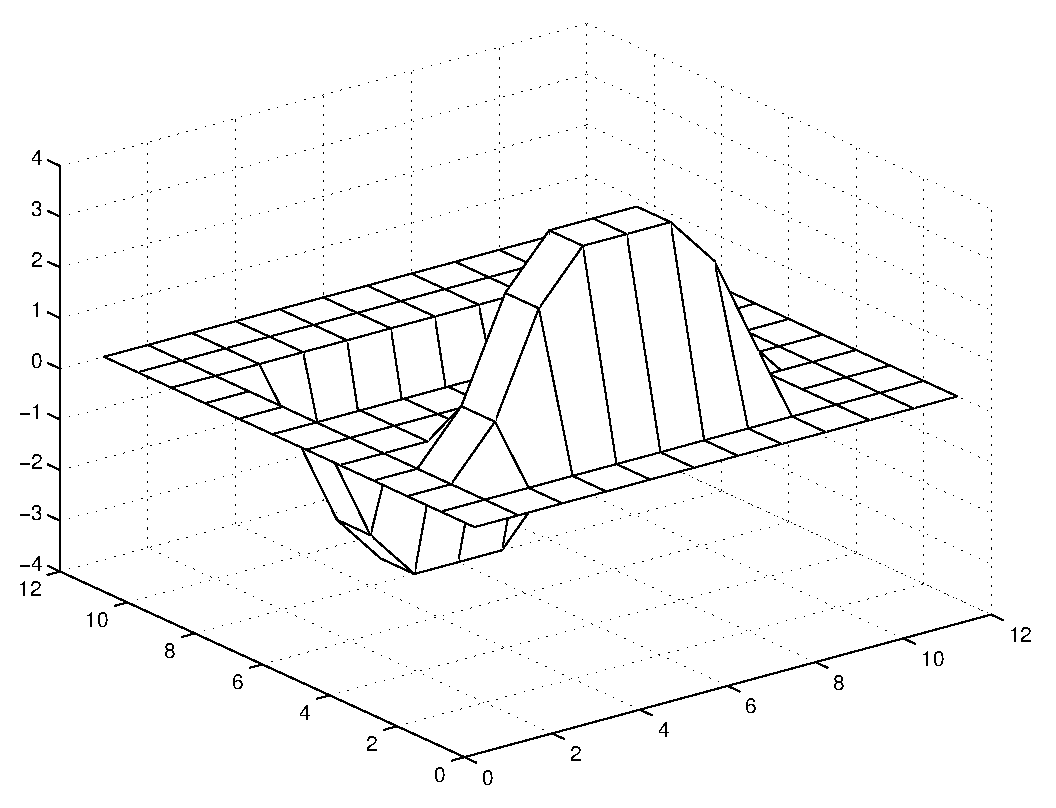
\includegraphics[width=4.5cm]{imtest3D.eps}
\end{tabular}
\caption{Imatge de nivell de gris i la seva representaci\'o tridimensional}
\label{imtest}
\end{center}
\end{figure}


Considerada d'aquesta manera, una imatge \'es equivalent a un conjunt de `muntanyes'
i `valls', on les primeres representen les zones clares de la imatge i els segons les
zones oscures. El filtre de gr\`a o aniquilador d'extrems elimina els pics m\'es 
punteguts i els avencs m\'es petits d'aquesta representaci\'o de la imatge.
Aquest pics i avencs s\'on, formalment, els extrems de la imatge.
El filtre dep\`en d'un \'unic par\`ametre qu\`e \'es el l'\`area dels extrems a eliminar ($A$).

La figura \ref{im1D} representa l'efecte del filtre de gr\`a per al cas uni-dimensional
i amb un par\`ametre $A=2$, qu\`e en aquest cas representa la longitud m\`axima dels 
extrems a eliminar.

\begin{figure}[htbp]
\begin{center}
\begin{tabular}{ccc}
\includegraphics[width=4.5cm]{im1D.eps} & & \includegraphics[width=4.5cm]{im1Dfiltrada.eps}
\end{tabular}
\caption{Funci\'o uni-dimensional i funci\'o filtrada amb un filtre de `gr\`a' de par\`ametre $2$}
\label{im1D}
\end{center}
\end{figure}

L'algoritme a implementar \'es el seg\"uent:
\begin{enumerate}
\item Trobar els p\'\i xels de la imatge qu\`e s\'on extrems locals (m\`axims
o m\'\i nims): $(i,j)$ \'es m\'\i nim local (resp. m\`axim) si $u(i,j) \leq u(i',j')$
(resp. $u(i,j) \geq u(i',j')$) $\forall i' \in \{i-1,i+1\}$, $j' \in \{j-1,j+1\}$. 
(Estam considerant aqu\'i 4-connectivitat).
\item Fer `cr\`eixer' cada un dels extrems trobats: trobar un grup de p\'\i xels connexos
tals que el seu nivell de gris m\'inim (resp. m\`axim) sigui major (resp. menor) que el
nivell de gris de tots els seus ve\"\i nats. El creixement de l'extrem es far\`a fins que es 
deixi de cumplir la condici\'o d'extrem o fins que el nombre de p\'\i xels en el grup 
sigui m\'es gran que el par\`ametre $A$.
\item Eliminar els extrems amb un nombre de p\'\i xels inferior o igual al par\`ametre $A$: 
a aquests p\'\i xels s'els assignar\`a un nou nivell de gris igual al del seu ve\"\i nat
amb nivell de gris m\'es alt (en el cas dels m\`axims) o amb nivell de gris m\'es baix 
(en el cas dels m\'inims).
\item Repetir el proc\'es per a tots els extrems de la imatge.
\end{enumerate}

\section{Detector de contorns cl\`assic (Marr-Hildreth, 1980)}

\noindent
{\bf Introducci\'{o}.} Dins el camp de la visi\'{o} per ordinador, el
tractament o an\`{a}lisi de les imatges \'{e}s una de les tasques fonamentals. Pensem en el cas de la
tomografia axial computada (TAC), la qual ens d\'{o}na informaci\'{o} sobre les estructures internes del
cos hum\`{a}. Poder entendre aquestes imatges requereix la identificaci\'{o} i modelitzaci\'{o} de les
superf\'{\i}cies dels objectes que s\'{o}n presents en les estructures en 3D. En el cas de les imatges per
sat\`{e}l$\cdot$lit, un dels problemes prov\'{e} del renou present en la imatge mateixa, potser degut a problemes
de captaci\'{o} o transmissi\'{o}. En aquest cas s'intenta fer un filtratge o preprocessament, intentant
eliminar aquest renou i conservar la informaci\'{o} inherent a la pr\`{o}pia imatge. Altres aplicacions
podrien ser el reconeixement autom\`{a}tic de les formes (reconeixement autom\`{a}tic de la signatura, el
problema de la videovigil\`{a}ncia, etc.), en el qual s'intenta extreure una s\`{e}rie de caracters que
ajudin en la identificaci\'{o} de l'objecte. Una imatge a nivell continu \'{e}s una funci\'{o} fitada que ens
mesura a cada punt la intensitat (o energia) de la llum que incideix en aquesta part de l'objecte.
\'{E}s evident que diferentes parts de la superf\'{\i}cie dels objectes reflecteixen diferents intensitats
de llum. Llavors la difer\`{e}ncia entre una fotografia o imatge natural i una imatge digital \'{e}s donada
pel tipus de codificaci\'{o}. Per posar una fotografia dins la mem\`{o}ria d'un ordinador es divideix la
imatge en petits trossos quadrats, que s'anomenen pixels i en cada un d'aquests trossos o pixels se
li associa un n\'umero que representa la llumnin\`{a}ncia. Normalment el negre est\`{a} codificat pel zero,
el 1 representa un color un poc menys negre, el 2 \'{e}s encara un poc menys negre que el 1, etc. Dins
la convenci\'{o} que s'utilitza en el m\'{o}n de la inform\`{a}tica, el 255 representa la codificaci\'{o} del color
blanc. Com a conseq\"{u}\`{e}ncia, operar amb imatges digitals vol dir operar amb matrius, ja que tota la
informaci\'{o} de la imatge \'{e}s continguda dins una matriu de n\'umeros.

\vskip 0.5 cm
\noindent
{\bf Pr\`{a}ctica del filtratge Multiescala} Detectar els diferents objectes dins una imatge vol dir
detectar els contorns dels objectes que hi apareixen. Pensem que una fotografia \'{e}s una projecci\'{o}
d'una escena $3D$ i per tant, \'{e}s complicat descriure els diferents objectes que hi s\'{o}n presents,
degut als efectes de les oclusions, ombres, etc. Un contorn va associat a punt de discontinu\"{\i}tat de
la imatge. Llavors, a nivell digital es treballa amb les ``m\`{a}scares" que no s\'{o}n m\'{e}s que
discretizacions num\`{e}riques d'operadors matem\`{a}tics. En el cas dels contorns d'una imatge $u$, direm
que el pixel $(i,j)$ pertany a un contorn si $\triangle u(i,j)=0$ i si $|\nabla u(i,j)|$ \'{e}s prou
gran. En aquest cas la m\`{a}scara, centrada al punt central $(i,j)$, on $i,j \in 0,1,\ldots,N$, que
ens descriu la laplaciana ve donada per

$$
A=\left(\begin{array}{ccc}
0 & 1 & 0 \\
1 & -4 & 1 \\
0 & 1 & 0 \end{array}\right)$$
 i la que descriu el gradient pel c\`{a}lcul de $u_x$ i $u_y$. L'aproximaci\'{o} de $u_x$ i $u_y$ ve donada
 per
$$
u_x=\left( \begin{array}{ccc} -1 & 0 & 1\\ -1 & 0 & 1 \\ -1 & 0 & 1 \end{array}\right)
$$ i la m\`{a}scara per al
c\`{a}lcul de la $u_y$
$$
u_y=\left(\begin{array}{ccc} -1 & -1 & -1 \\ 0 & 0 & 0 \\ 1 & 1 & 1 \end{array}\right)$$
 Llavors $\nabla u=(u_x,u_y)$.
\newline La teoria del "scale-space" o espai-escala, introduida per Marr-Witkin (1982),
La idea b\`{a}sica \'{e}s que la informaci\'{o} de la imatge est\`{a} continguda en diferents escales que ens donen
les diferents caracter\'{\i}stiques de la imatge a diferents nivells de resoluci\'{o}. Per aix\`{o}, farem un
filtratge de la imatge en diferents nivells i en cada nivell, calcularem els contorns o
carater\'{\i}stiques associades a dit nivell.
\newline
 Un dels filtres m\'{e}s comuns ve donat per la convoluci\'{o} de la imatge amb la funci\'{o} gaussiana. En
aquest cas es pot construir una m\`{a}scara que centrada al pixel $(i,j)$ simuli num\`{e}ricament la
convoluci\'{o} amb la gaussiana. B\`{a}sicament aquesta operaci\'{o} ens d\'{o}na una mitja ponderada al voltant
del pixel $(i,j)$, i per tant, quan fem aquesta operaci\'{o},
 ``regularitzem'' o ``suavitzem'' la imatge. Definim una successi\'{o} de m\`{a}scares ponderades de la
 seg\"{u}ent manera:
 $$
M_1=\frac{1}{6}\left(\begin{array}{ccc} 0 & 1 & 0\\ 1 & 2 & 1\\ 0 & 1 & 0 \end{array}\right).$$
 $$
M_2=\frac{1}{16}\left(\begin{array}{ccc} 1 & 2 & 1 \\ 2 & 4 & 2 \\ 1 & 2 & 1 \end{array}\right).$$
 $$
M_3=\frac{1}{36}\left(\begin{array}{ccccc} 0 & 0 & 1 & 0 & 0 \\ 0 & 2 & 4 & 2 & 0 \\ 1 & 4 & 8 & 4 & 1 \\ 0
& 2 & 4 & 2 & 0 \\ 0 & 0 & 1 & 0 & 0 \end{array}\right).$$
 $$
M_4=\frac{1}{80}\left(\begin{array}{ccccc} 0 & 1 & 2 & 1 & 0 \\ 1 & 4 & 8 & 4 & 1 \\ 2 & 8 & 16 & 8 & 2 \\ 1
& 4 & 8 & 4 & 1 \\ 0 & 1 & 2 & 1 & 0 \end{array}\right).$$ Tamb\'{e} es podria pensar de fer realment la
mitja dels valors, i no la mitja ponderada, com \'{e}s el cas de la gausiana. En aquest cas el
suavitzat es faria m\'{e}s r\`{a}pid, ja que no hi ha informaci\'{o} privilegiada de cap dels pixels de
l'entorn. 
\vskip 0.2 cm
\newpage 
{\bf Part 1: Filtratge gaussi\`{a} (sense direccions privilegiades)} \vskip 0.1
cm (i) Sigui $I_0$ la imatge original, i fem la convoluci\'{o} amb les diferents m\`{a}scares introdu\"{\i}des
abans. S'obtenen les noves imatges $I_1, I_2, I_3, I_4$. \vskip 0.1 cm (ii) Per a cada imatge
$I_i$, calculeu els seus contorns, \'{e}s a dir: Passeu la m\`{a}scara $u_x$, $u_y$ i calculeu la imatge
del m\`{o}dul del valor absolut $Mod_{i}=u_x^2+u_y^2$. Feu el mateix amb la laplaciana i obtindreu
$L_i$. Llavors definiu la nova imatge dels contorns com a $Co_i(i,j)$, on $Co_i(i,j)=0$ si tenim un
contorn, \'{e}s a dir, si $Mod_{i}(i,j) > K$ i $|L_i(i,j)|<\epsilon$, on $k, \epsilon$ s\'{o}n par\`{a}metres
prefixats, i $Co_i(i,j)=255$ en cas contrari (de no contorn). \vskip 0.2 cm {\bf Part 2: Filtratge
condicionat} \vskip 0.1 cm Definim les seg\"{u}ents masc\`{a}res ponderades per direccions, on entenem que
a nivell discret, tenim 4 direccions principals.
 $$
v_1=\frac{1}{4}\left(\begin{array}{ccc} 0 & 0 & 0 \\ 1 & 2 & 1 \\ 0 & 0 & 0 \end{array}\right).$$
 $$
v_2=\frac{1}{4}\left(\begin{array}{ccc} 0 & 0 & 1 \\ 0 & 2 & 0 \\ 1 & 0 & 0 \end{array}\right).$$
 $$
v_3=\frac{1}{4}\left(\begin{array}{ccc} 0 & 1 & 0 \\ 0 & 2 & 0 \\ 0 & 1 & 0 \end{array}\right).$$
 $$
v_4=\frac{1}{4}\left(\begin{array}{ccc} 1 & 0 & 0 \\ 0 & 2 & 0 \\ 0 & 0 & 1 \end{array}\right).$$ Per tant podem
definir un partici\'{o} del domini de les direccions de la seg\"{u}ent manera $D_1=[-\frac{11}{8}\pi,
-\frac{3}{8}\pi], D_2=[-\frac{3}{8}\pi, -\frac{1}{8}\pi], D_3=[-\frac{1}{8}\pi, \frac{1}{8}\pi],
D_4=[\frac{1}{8}\pi, \frac{3}{8}\pi], D_5=[\frac{3}{8}\pi, \frac{5}{8}\pi]$. Llavors donada una
direcci\'{o} $v$, existeixen dues direccions, les de m\'{e}s a prop $v_i, v_j$ tal que $v=\theta_1 v_1+
\theta_2 v_2$, on $\theta_1+\theta_2=1$. Feu els mateixos passos que per la pr\`{a}ctica del filtratge
gaussi\`{a}.

\vskip 1.2 cm
La informaci\'o necess\`aria per implementar els algoritmes
es subministrar\`a a l'alumne en forma de fotoc\`opies 
({\it Digital Image Processing}, Gonzalez and Woods, Ed. Addison-Wesley, 1993. pp.416-425).

\section{Segmentaci\'o d'imatges per creixement de regions ({\it region growing})}
\noindent
{\bf Pr\`{a}ctica de Segmentaci\'{o}} L'operaci\'{o} de segmentaci\'{o} intenta dividir la imatge en les diferents
regions disjuntes homeg\`{e}nies respecte a una propietat(segons un criteri de similitud (nivell de
gris, textura, color, etc)), generalment relacionada amb el valor del nivell de gris (Per exemple,
un criteri podria ser que la difer\`{e}ncia absoluta en nivell de gris entre la "llavor" i el pixel
candidat, no exced\'{\i}s d'un 10 per cent de la difer\`{e}ncia entre el nivell de gris m\`{a}xim i el m\'{\i}nim de
la image sencera, i que el pixel candidat fos un ve\"{\i}nat de la regi\'{o} que hi formar\`{a} part). El m\`{e}tode
m\'{e}s simple \'{e}s l'anomenat creixement de regions o ``region growing''. \newline {\bf Part 1} Feu un
programa per segmentar imatges, basat en aquest model. Gen\`{e}ricament l'algorisme seria:
\newline
a) Comen\c car amb que tot pixel \'{e}s una regi\'{o} diferent.
\newline
b) Fer una uni\'{o} de tots els parells de regions que en ``adjuntar-les'' millora la segmentaci\'{o}, a
partir d'uns pixels inicials o llavors, per la caracter\'{\i}stica o propietat que agafam. Per exemple,
si el valor mig del nivell de gris difereix tan sols en un valor $\lambda =2$. Pensau en altres
criteris.
\newline
c) Agafar un $\lambda$ m\'{e}s gran i iterar el proc\'{e}s.
\newline
{\bf  Formulaci\'{o} variacional} Existeix una formulaci\'{o} variacional del problema, suposant que les
imatges que s'obtenen s\'{o}n constants a trossos. Aquest es un m\`{e}tode que minimitza una certa energia,
conegut com el funcional de Mumford-Shah:
$$E(u,K)=\lambda^2 \int_{K} d\sigma + \int_{\Omega-K}(u-u_{0})^2dx$$
on $u_{0}$ \'{e}s la imatge original. En aquest funcional, $K$ \'{e}s el la uni\'{o} de corbes en que segmenta
la imatge, $\Omega$ \'{e}s el domini de la imatge, $u_{0}$ \'{e}s la imatge incial que es vol segmentar i
$u$ \'{e}s la imatge segmentada en el conjunt de corbes $K$.
 El primer terme minimitza la
llarg\`{a}ria de les fronteres de les regions mentre que el segon s'anomena terme de fidelitat, ja que
no permet que la imatge resultant de la segmentaci\'{o} sigui molt ``diferent'' de la original.
\newline {\bf Part 2} d) Feu un programa basat en un m\`{e}tode num\`{e}ric que ens resol de manera iterativa
el problema d'optimitzaci\'{o}, per exemple, del gradient, on poguem minimitzar el funcional, i per
tant, trobar la soluci\'{o} aproximada, segons $\lambda$, de la segmentaci\'{o} de la imatge original.

\vskip 1.2cm
La informaci\'o necess\`aria per implementar els algoritmes
es subministrar\`a a l'alumne en forma de fotoc\`opies 
({\it Digital Image Processing}, Gonzalez and Woods, Ed. Addison-Wesley, 1993. pp.458-462).

\end{document}
